\section{Theory}
<<<<<<< HEAD

Rossby waves are described in what known as the Quasi Geostrophic (QG)
framework. The primary scaling assumption in QG theory is that the Rossby number
is much less that one. The Rossby number which can be obtained by scaling the
momentum equation is defined as the following:
\cref{eq:Rnumber},
\begin{equation}\label{eq:Rnumber}
    R = \frac{U}{fL}
\end{equation}
Where $U$ is characteristic magnitude of the horizontal velocity, $f \sim 10^{-4}$
is the Coriolis parameter and $L$ the characteristic horizontal length scale.
From the assumption about the Rossby number it is evident that the horizontal
length scales has to be large. A feature of large scale motion in the atmosphere
and ocean is that there tends to be a balance between the pressure gradient
force and Coriolis acceleration acting perpendicular to the velocity vector.
\begin{equation}\label{eq:geostrophic}
    fu = -\frac{1}{\rho}\pdv{p}{y} \quad fv = \frac{1}{\rho}\pdv{p}{x}
\end{equation}
The issue with a purely geostrophic framework \cref{eq:geostrophic} is that
there is no development of the motion.

In QG-theory velocities is
separated into a geostrophic and ageostrophic component $\mathbf{v} = \mathbf
{v_g} +\mathbf{v_a}$. The geostrophic velocities are
non-divergent and can consequently be written in terms of a steam function.
It is the ageostrophic wind which are responsible for the
horizontal divergence. Even though the ageostrophic velocities
are small compared to the geostrophic, they are important since
they governs the rising and sinking in the atmosphere.

The quasi geostrophic potential vorticity equation \cref{eq:QG_vort} can be
derived from the shallow water equations \textbf{CITE Joe}, following the
previously discussed
assumptions.
=======
\subsection{The barotropic Rossby wave equation}
The first step towards the BRWE is to linearise the vorticity equation 
\cref{eq:QG_vorticity}. If we suppose that the flow can be represented by a
mean flow plus some small perturbation: 
\begin{equation}\label{eq:VeloctiyPertubation}
    \begin{split}
    u = U + u' \quad  |U| >> u' \\
    v = V + v' \quad  |V| >> v'
    \end{split}
\end{equation}
Then the vorticity of the mean and the perturbation is: 

\begin{equation}\label{eq:VortPertubation}
    Z = \pdv{V}{x} - \pdv{U}{y} \; , \quad \zeta' = \pdv{v'}{x} - \pdv{u'}{y} 
\end{equation}
To linearise the Coriolis parameter, we expand $f$
around a reference latitude $\theta_0$: 
\begin{equation}
    f \approx f_0 + \beta y
\end{equation} 
where $f_0 = 2\Omega \sin(\theta)$, $\beta = 2\cos (\theta_0)/R_e$ and $R_e$ is
the radius of the earth. This linearisation of the Coriolis parameter is
commonly referred to as the $\beta-\mathrm{plane}$ approximation.
>>>>>>> master

\begin{equation}
    \pdv{\zeta'}{t} + (U+u')\pdv{\zeta'}{x} + (V+v')\pdv{\zeta'}{y} + \bvec{U} 
    \cdot \nabla q_s + u' \pdv{q_s}{x} + v' \pdv{q_s}{y} = 0     
\end{equation}
\begin{equation}\label{eq:q_s}
    q_s = Z + f_0 + \beta y
\end{equation}
Then mean flow $\bvec{U}$ is geostrophic, consequently the flow will be parallel
to the contours of stationary potential vorticity $q_s$, ergo $\bvec{U} \cdot
\nabla q_s = 0$. The perturbations are assumed to be so weak that perturbations
advecting perturbations can be neglected. Thus we get the following linearised
barotropic vorticity equation:

\begin{equation}
    \pdv{\zeta '}{t} + U\pdv{\zeta'}{x} + V\pdv{\zeta'}{y} + \beta v' = 0
\end{equation}

We will drop the primes from here on. Then if we suppose that the velocity of
the mean flow is zero, and express the velocities in terms of the streamfunction
$\psi$, $u = -\pdv{\psi}{y}$, $v = \pdv{\psi}{x}$ and $\zeta = \nabla_H^2 \psi
$.The equation we end up with is the barotropic Rossby wave equation
\cref{eq:barotropicRossby} in the absence of a mean flow. 

\begin{equation}\label{eq:barotropicRossby}
    \pdv{}{t} \nabla_H^2 \psi + \beta \pdv{\psi}{x} = 0
\end{equation}

\subsection{Analytic expression of phase velocities}



We assume the following periodic solution \cref{eq:waveSolution} and
insert this into the barotropic Rossby wave equation \cref{eq:barotropicRossby}.
\begin{equation}\label{eq:waveSolution}
    \psi = A\cos{(2n\pi x /L - \omega t)}
\end{equation}
Using the one dimensional vorticity $\zeta_x = \pdv{v}{x} = \pdv[2]{\psi}{x}$

\begin{equation}
    \pdv{}{t} \left(-A (2n\pi/L)^2  \cos{(2n\pi x/L - \omega t)}\right) - \beta
     (2n\pi/L) A \sin{(2n x\pi/L - \omega t) = 0}
\end{equation}

\begin{equation}
    -(2n\pi/L)\omega \cancel{A\sin{(2n x\pi/L - \omega t)}} - \beta
    \cancel{A\sin{(2 xn\pi/L - \omega t)}} = 0
\end{equation}

\begin{equation}
    (2n\pi / L) \omega = \beta
\end{equation}

\begin{equation}\label{eq:omega1}
    \omega = \frac{-\beta L}{2n\pi}
\end{equation}

The phase speed of the Rossby wave can be derived by considering the phase of
the wave \cref{eq:phase}.
\begin{equation}\label{eq:phase}
    \theta = \frac{n \pi x}{L} - \omega t
\end{equation}
Then peak of the wave would be at $\theta = 2\pi$, where $\psi = A\cos{(2\pi)}$.
In therms of the atmospheric motion this peak would correspond to would
correspond to high pressure point. To get the motion of this point we can solve
\cref{eq:phase} for x, $x=\theta L / 2n \pi + \omega t L / 2n \pi$ and then
obtaining the phase speed by taking the time derivative.
\begin{equation}
    c = \dv{x}{t} = \frac{\omega L}{2n\pi}
\end{equation}
Inserting the expression for $\omega$ obtained previously \cref{eq:omega1}, we
get the following expression for the phase speed.
\begin{equation}\label{eq:Phase-speed1}
    c = \frac{-\beta L^2}{(2n\pi)^2}
\end{equation}
Then following \cref{eq:Phase-speed1} the Rossby wave will propagate
toward the west.
Next we assume a more realistic wavelike solution of \cref{eq:barotropicRossby}
where the amplitude of the wave is also a function of $x$. We
require there to be no flow at the endpoints, which we can enforce with simple
Dirichlet conditions $\psi= 0$ at $x=0$ and $x=L$.
\begin{equation}\label{eq:waveSolution2}
    \psi = A(x)\cos{(kx-\omega t)}
\end{equation}
Inserting \label{eq:waveSolution2} into the barotropic Rossby wave equation
\cref{eq:barotropicRossby} and then differentiating we get the following
equation:

\begin{equation}\label{eq:step1}
    \begin{split}
    \sin{(kx-wt)\left(\omega(A''(x)-k^2A(x))- \beta A(x)\right)} \\
    + \cos{(kx - \omega t)}\left(\omega 2kA'(x) +\beta A'(x)\right) = 0
    \end{split}
\end{equation}
The terms in front of the cosine and sine has to be zero, which means that we
can split equation in to two parts. The equation for the sine and cosine terms
respectively.

\begin{equation}\label{eq:sine-terms}
    \omega A''(x) -\omega k^2 A(x) - \beta A(x) = 0
\end{equation}
\begin{equation}\label{eq:cos-terms}
    \omega 2 k A'(x) + \beta A'(x) = 0
\end{equation}

Solving the equation for the cosine terms \cref{eq:cos-terms} with respect to
$\omega$:
\begin{equation}
    \omega = -\frac{\beta}{2k}
\end{equation}
Inserting the expression for omega into \cref{eq:sine-terms} and solving the ODE
give the following expression for $A(x)$
\begin{equation}\label{eq:A_x}
    A(x) = C_1 \cos{(kx) + C_2 \sin{(kx)}}
\end{equation}
Imposing the boundary condition at $x=0$ requiring $C_1$ to be zero ruling
out the cosine term in \cref{eq:A_x}. Imposing the boundary condition $\psi=0$
at $x=L$ yields the following expression for A(x).
\begin{equation}
    A(x) = \sin{\left(\frac{n\pi}{L} x \right)}
\end{equation}
Then final solution becomes:
\begin{equation}
    \psi = \sin{\left(\frac{n\pi}{L} x \right)} \cos{(kx - \omega t)}
\end{equation}
The phase speed can be calculated in the same manner as previously and inserting
the previously obtained expressions for $k$, $k=\frac{n\pi}{L}$ and $\omega$,
$\omega = -\frac{\beta}{k}$.
\begin{equation}
    c = \dv{x}{t} = \frac{\omega}{k} = -\frac{\beta}{2k^2} = -\frac{\beta L^2}{2 n^2 \pi^2}
\end{equation}

\subsection{Scaling}

To make the vorticity equation dimensionless we scale it using $x = \tilde{x} L $ and $t = \frac{\tilde{t}}{L \beta}$. The dimensionless phase speed is then $\frac{d\tilde{x}}{d\tilde{t}} = \frac{1}{\beta L^2} c$. For wavenumber two this gives us phase speeds of
$0.0063$ for the periodic case and $c = 0.012665$ for the bounded case.

After scaling \cref{eq:gov_vort} we get \cref{eq:vort_scaled} which we
will solve numerically.

\begin{equation}
  \pdv{\zeta}{\tilde{t}} + \pdv{\psi}{\tilde{x}} = 0
  \label{eq:vort_scaled}
\end{equation}


\subsection{Implementation and testing}

\begin{algorithm}
  \SetAlgoLined
  initialize $\zeta$ and $\psi$ using sine or gaussian\\
  \For{t=0; t<\text{timesteps}; t++}{
    advance $\zeta$ one timestep \\
    update $\psi$ using jacobis method
  }
  \caption{General algorithm for solving the vorticity equation.}
  \label{algo:vort}
\end{algorithm}


The general algorithm for solving the vorticity equation is outlined in
\cref{algo:vort}. We implemented two methods for advancing $\zeta$ using centered
(\cref{eq:centered}) and forward (\cref{eq:forward}) differences.
For the planetary vorticity advection term we used centered differences.
This lead to the timestepping schemes \cref{eq:advance_centered} and
\cref{eq:advance_forward}.


\begin{equation} \label{eq:centered}
  \pdv{\zeta}{t} \approx \frac{\zeta_{}^{n+1} - \zeta_{}^{n-1}}{2 \Delta t}
\end{equation}

\begin{equation} \label{eg:forward}
  \pdv{\zeta}{t} \approx \frac{\zeta_{}^{n+1} - \zeta_{}^{n}}{\Delta t}
\end{equation}


\begin{equation} \label{eq:advance_centered}
  \zeta_{i}^{n+1} = \zeta_{i}^{n-1} - \frac{\Delta t}{2 \Delta x}
    (\psi_{i+1}^{n} - \psi_{i-1}^{n})
\end{equation}


\begin{equation}   \label{eq:advance_forward}
  \zeta_{i}^{n+1} = \zeta_{i}^{n} - \frac{\Delta t}{\Delta x} (\psi_{i+1}^{n} - \psi_{i-1}^{n})
\end{equation}


After advancing the vorticity one timestep we run adjust the stream function
according to ref eq??. We do this by solving the poisson equation using
jacobis method. The method requires a convergence parameter for deciding when to
stop iterating. To set this we tested with two analytical solutions of poissons
equation, one bounded, one periodic. \Cref{fig:error_jacobi} shows the absolute
error of jacobis method compared to these solutions.
As the convergence parameter is lowered the method performs better for larger grids.
Since we are using close to 40 grid points for our simulations we ended up
setting the convergence parameter to 10$^{-8}$.

\begin{figure}[htp]
  \centering
  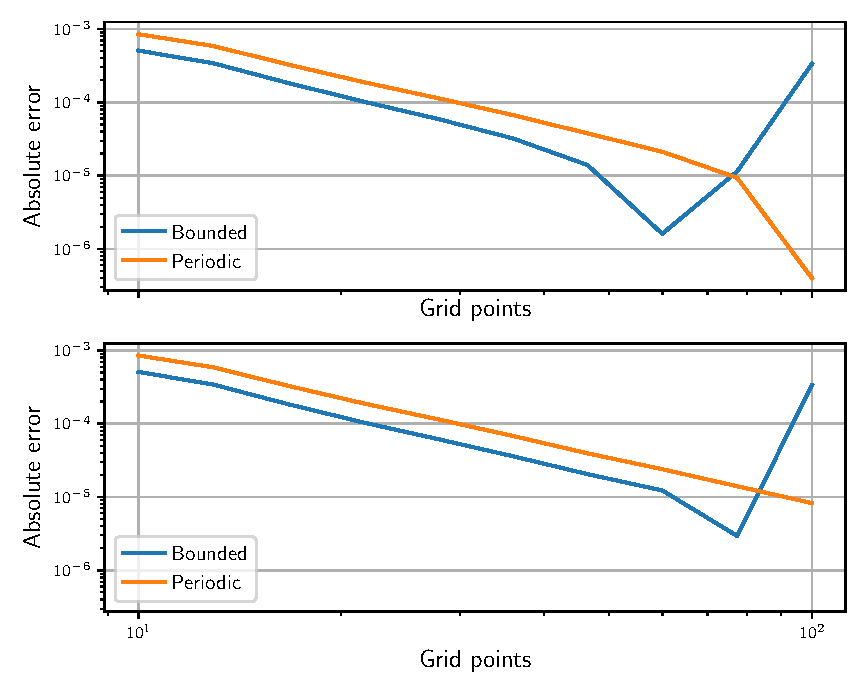
\includegraphics[width=\textwidth]{../figures/error_jacobi.pdf}
  \caption{Absolute error of jacobis method
  compared to analytical solutions of poissons equation. Convergence parameter set to (from top to bottom) 10$^{-6}$, 10$^{-8}$ and 10$^{-10}$.
  The absolute error should have a slope of -2 in loglog space since we use
  a centered second order scheme with truncation error proportional to $(\Delta x)^2$.
  The larger values of the convergence parameter has the correct slope for small
  grids, but performs worse with larger grids. As the parameter is lowered the
  slope is correct for increasingly larger grids.}
  \label{fig:error_jacobi}
\end{figure}


\begin{figure}[htp]
  \centering
  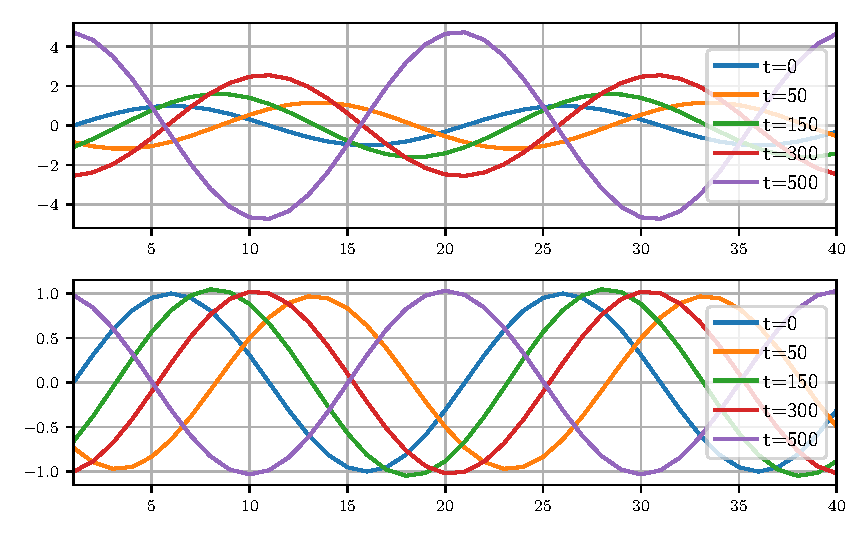
\includegraphics[width=\textwidth]{../figures/compare_dt_1.pdf}
  \caption{Comparison of solutions at different times using forward (top) and
  centered (bottom) differences in time. The solution using forward differences
  blows up quickly while the one using central differences does not.}
  \label{fig:compare}
\end{figure}


\Cref{fig:compare} shows the blow up of the numerical solution with forward
time step with $\Delta t = 1$ and $\Delta x = 0.025$ for the periodic case.
With a central difference in time the solution stays stable.
All the rest of the plots are done using the central difference.
